\documentclass[class=article,border=5pt,tikz]{standalone}
\usetikzlibrary{backgrounds, scopes, positioning}
\usetikzlibrary{matrix}

\tikzset{
    mygrid/.style={
        matrix,
        inner sep=1pt,
        column sep=-\pgflinewidth,
        row sep=-\pgflinewidth,
        matrix of nodes,
        nodes in empty cells,
        nodes={draw=gray, anchor=center, inner sep=.3333em, minimum size=5mm}
    }
}

\begin{document}

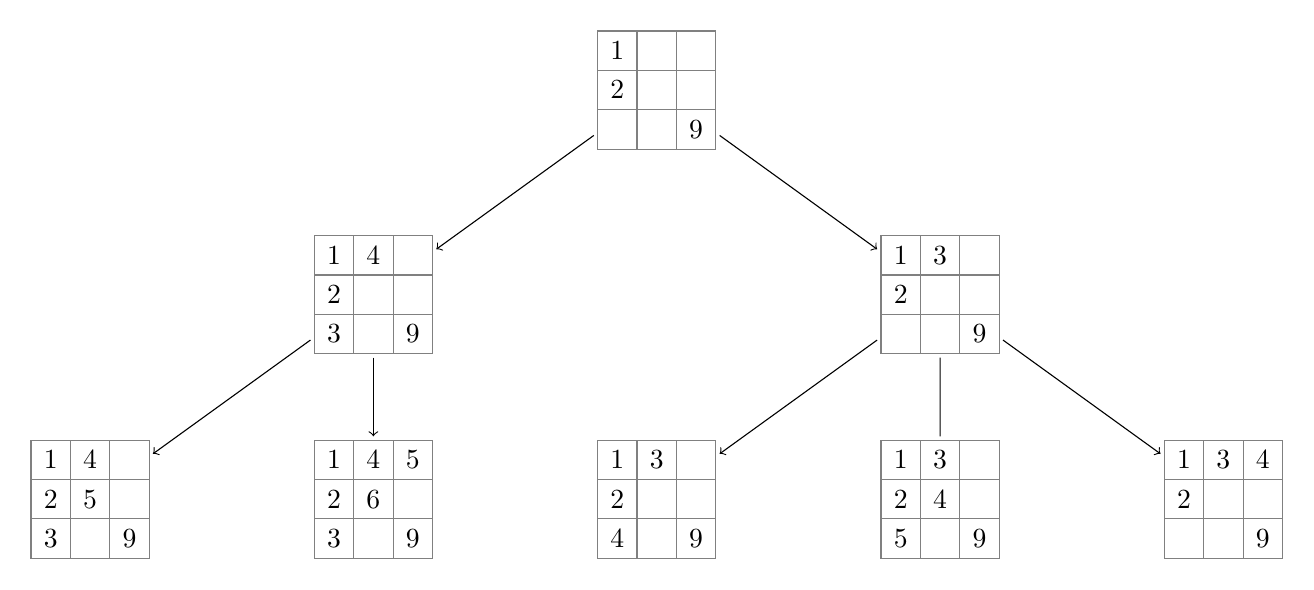
\begin{tikzpicture}[node distance = 10mm and 20mm]
\node[mygrid]                   (A) {1&&\\2&&\\&&9\\};
\node[mygrid, below left=of A]  (B) {1&4&\\2&&\\3&&9\\};
\node[mygrid, below right=of A] (C) {1&3&\\2&&\\&&9\\};
\node[mygrid, below left=of B]  (D) {1&4&\\2&5&\\3&&9\\};
\node[mygrid, below =of B]      (E) {1&4&5\\2&6&\\3&&9\\};
\node[mygrid, below left=of C]  (F) {1&3&\\2&&\\4&&9\\};
\node[mygrid, below =of C]      (G) {1&3&\\2&4&\\5&&9\\};
\node[mygrid, below right=of C] (H) {1&3&4\\2&&\\&&9\\};

\scoped[on background layer]
    \draw[->] (A) edge (B) (A) to (C);
    \draw[->] (B) edge (D) (B) to (E);
    \draw[->] (C) edge (F) (C) to (G) (C) to (H);
\end{tikzpicture}

\end{document}